% Chapter 6

\chapter{Marco Teórico} % Write in your own chapter title
\label{Chapter6}
\lhead{Capítulo 6. \emph{Marco Teórico}} % Write in your own chapter title to set the page header
\section{Estado del Arte}

\subsection{Computación de Borde}

El IoT, definido como una red distribuida de dispositivos heterogéneos (sensores, actuadores y procesadores) que intercambian mensajes entre ellos sin intervención humana, ha cobrado particular interés por parte de los investigadores, dado que miles de millones de dispositivos se estarán comunicando en un futuro cercano. La Figura \ref{fig:IoTEvol}, muestra la tendencia de la capacidad de procesamiento y la cantidad de servicios que el IoT puede ofrecer, a la par que también aumentan los retos de seguridad y administración de los datos \citep{li2015internet,stojmenovic2014fog}.
 
\begin{figure}[!ht]
	\centering
		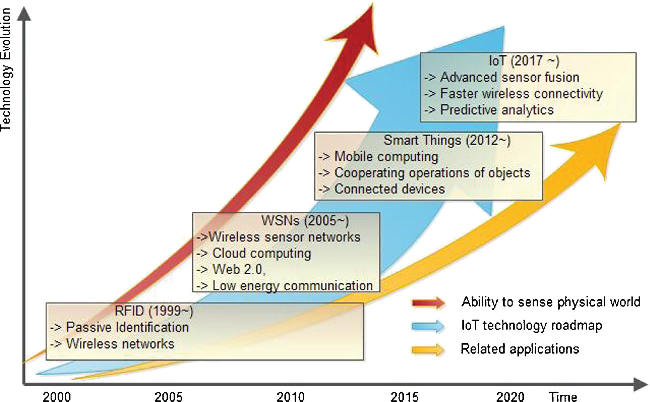
\includegraphics[scale=1.2]{Figures/IoTEvol}
	\caption{Evolución y aplicaciones de IoT\cite{li2015internet}.}
	\label{fig:IoTEvol}
\end{figure}

Con el incremento en la cantidad de servicios, también surgen otras necesidades. Algunas de ellas y quizá las más críticas en la arquitectura pensada para IoT, son la latencia de los datos y el rendimiento del sistema \cite{bonomi2012fog}. Por ello, se propone llevar algunos de los servicios de la nube más cerca del nivel al que se encuentran los datos así como emplear múltiples niveles, según las necesidades de las diferentes aplicaciones, como lo muestra la Figura \ref{fig:IoTDist}. En el caso del nivel \textit{Extremo} ó \textit{MIST}, se tienen niveles de procesamiento bajos; en este nivel, son los mismos nodos sensores y actuadores, los que toman decisiones operativas a un nivel muy bajo dadas las limitaciones en los procesadores que requieren para funcionar. A nivel de \textit{Borde} ó \textit{FOG}, se tiene mayor potencia de cálculo permitiendo realizar labores de almacenamiento, analítica, toma de decisiones, etc. Esto es posible, dado que en algunas aplicaciones, el dispositivo de borde, también conocido como Gateway, hace la labor de establecer un puente entre el extremo y la nube, contando con una radio potente y una conexión a Internet y alimentación eléctrica estables; es por estas necesidades que el gateway dentro de su concepción debe contar con hardware más potente que los demás dispositivos. Finalmente, sobre la última capa se encuentra la \textit{Nube} ó \textit{CLOUD}, el cual es el pilar más importante del Internet de las Cosas, ofreciendo múltiples servicios, con recursos prácticamente ilimitados en procesamiento, capaz de escalar dinámicamente conforme las necesidades lo requieran \cite{bonomi2014fog}.

\begin{figure}[!ht]
	\centering
		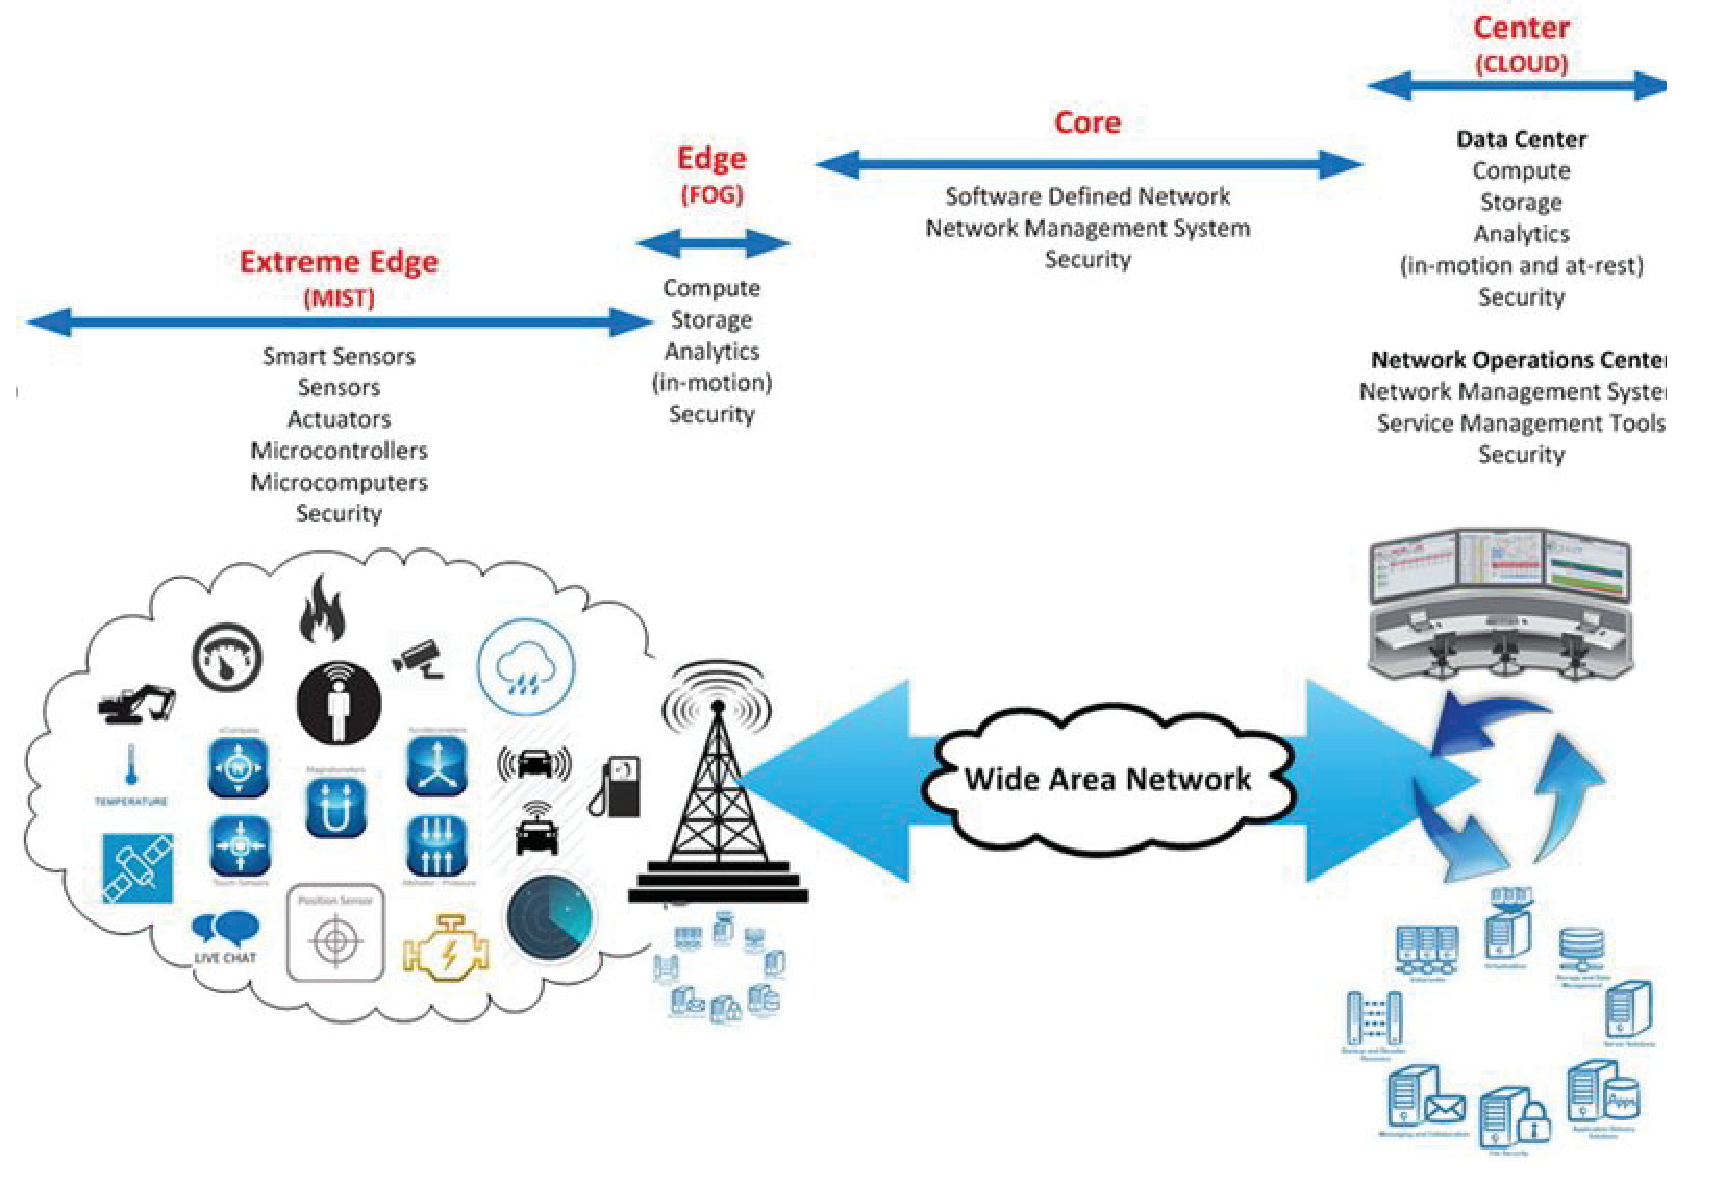
\includegraphics[scale=0.5]{Figures/IoTDist}
	\caption{Distribución del Internet de las Cosas (Operación)\cite{bonomi2012fog}.}
	\label{fig:IoTDist}
\end{figure}

Entonces, como se sugiere, la computación de borde está orientada a comunicación entre dispositivos, con una orientación a un almacenamiento y toma de decisiones eficientes. Esto implica directamente reducción en tiempo de procesamiento, almacenamiento, visualización y manejo de los datos como se muestra en la Figura \ref{fig:IoTFogGr}. 

Al final, la nube como el pilar fundamental, ofrece potencia de cálculo y por ende más servicios \cite{madsen2013reliability}, pero algunas de las aplicaciones únicamente requieren parte de estos servicios, que pueden ser resueltos en el borde por un gateway. Las aplicaciones que hacen uso de la computación de borde pueden ser de cualquier tipo; por ejemplo, encontramos modelos de programación para aplicaciones que requieran procesamiento de borde a gran escala \cite{hong2013mobile}, Gateways inteligentes capaces de enrutar de mejor manera los paquetes de red que tienen como destino la nube \cite{aazam2014fog}, modelos de \textit{centros de datos} para el procesamiento de datos efectivos en el borde \cite{aazam2015fog}, QoS distribuido dentro de la red de IoT \cite{cardellini2015distributed}. Como se ve, el concepto es ampliamente usado, pero el terreno sobre la aceleración por hardware sigue sin ser explorado, dadas las complicaciones que requiere su programación. Con sintetizadores de alto nivel apenas madurando, se espera avanzar hacia la creación de APIs ó middlewares que permitan a los desarrolladores incrementar la potencia de cálculo en el borde como lo sugieren las patentes \citep{subramanian2016dynamic,zhu2013improving}.

\begin{figure}[!ht]
	\centering
		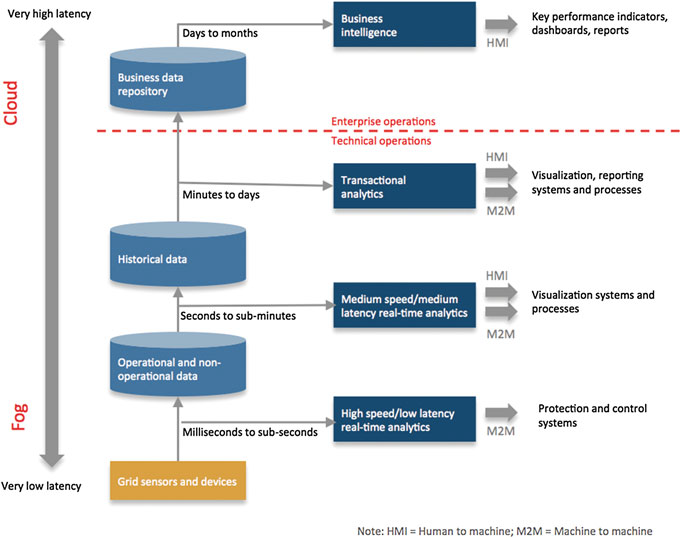
\includegraphics[scale=1.2]{Figures/IoTFogGr}
	\caption{Escalas de tiempos de servicios de la computación de borde vs la nube\cite{bonomi2014fog}.}
	\label{fig:IoTFogGr}
\end{figure}

\subsection{Computación Consciente del Contexto}

Cuando se habla de grandes cantidades de datos recolectada por miles de sensores dentro de un esquema de IoT, se pone sobre la mesa una pregunta: ¿Cómo interpretar los datos?. Es importante notar que por más información que se tenga disponible, si no se analiza, interpreta y entiende dentro de un contexto dado, esta información no tiene valor alguno.

La computación consciente del contexto, vista desde una perspectiva de IoT, propone una forma de mediar con la información desde diferentes flancos. Actualmente hablamos de la implementación de soluciones middleware capaces de añadir recursos que se encarguen de abstraer, fusionar y comprimir los datos, además de añadir servicios como QoS, paradigmas de programación, adaptabilidad, escalabilidad, recursos de hardware y lo más importante, seguridad de los datos \citep{molla2006survey}.

\begin{figure}[!ht]
	\centering
		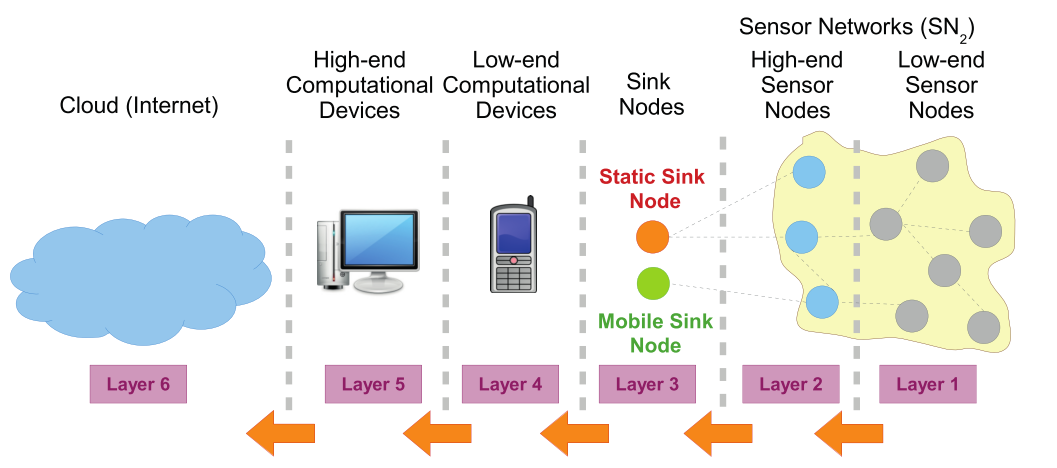
\includegraphics[scale=0.75]{Figures/Structure_of_a_sensor_network}
	\caption{Red de sensores estructurada por capas \citep{perera2014context}.}
	\label{fig:IoTWSN2Cloud}
\end{figure}

La Figura \ref{fig:IoTWSN2Cloud} ofrece una vista general de la forma como se distribuye una red de sensores por capas, desde los elementos más básicos hasta los más complejos. En las primeras tres capas se observa el flujo de datos que va desde los dispositivos menos potentes hasta los más potentes en la capa 3, que muchas veces hacen las veces de enrutadores de borde de red. En las capas 4 y 5 se tienen dispositivos computacionalmente mucho más potentes; estos son conocidos como Gateways, capaces de llevar la información del campo hacia la nube. Finalmente, se tiene la Nube en Internet, donde la información capturada puede ser transformada y procesada para su análisis. Cada una de las capas cumple un rol específico en el que la eficiencia es la clave\citep{sho2008ttcg}. Nótese que el procesamiento se podría realizar entre las dos primeras capas reduciendo considerablemente el costo de las comunicaciones; sin embargo, las limitaciones en capacidad de cómputo y energéticas impedirían realizar un análisis detallado de la información recolectada por la red.

En función de esta necesidad, los investigadores definieron siete grandes características que permiten enmarcar una solución para el IoT dentro del contexto de la computación consciente del contexto que, necesariamente, dadas las condiciones, deben ser realizadas entre las capas cuatro a seis \citep{sundmaeker2010vision}. Estas son: inteligencia, arquitectura, sistemas complejos, magnitud, tiempo, espacio y ``Todo como un Servicio'' o ``All as a Service''. Algunas de estas cobran particular interés, como inteligencia, pues determina que para usar la información recolectada por diferentes fuentes en crudo se debe transformar para lograr lo que se denomina \textit{información de alto nivel}, que lo que quiere decir es que esta información nueva enriquecida y puesta en un contexto, pueda ser usada como insumo para otro tipo de operaciones. Otra de las características que cobra particular interés es la de tiempo, pues dados los altos volúmenes de transacciones de datos se hacen necesarios mecanismos que permitan operar en tiempo real, siendo una restricción importante cuando se modela una solución de este tipo. 
%tek
%
% > siete características versus seis enunciadas
%
% > inteligencia, arquitectura, sistemas complejos, magnitud, tiempo, espacio

A partir de este punto, se introduce el concepto \textit{``Principios Administrativos de Diseño Consciente del Contexto"}, que básicamente se define como, los requerimientos para la aplicación de un middleware consciente del contexto de operación, que se encuentre en capacidad de analizar, transformar e interactuar con el medio para darle sentido a la información \citep{martin2010automatic,ramparany2007open,bernardos2008data}. Uno de los requerimientos más tangibles es el llamado \textit{optimización de recursos}, el cual implica que, cualquier mejora en los recursos de procesamiento, por más pequeña que sea, tendrá un gran impacto en el procesamiento dados los altos volúmenes de información que el IoT puede llegar a procesar.

Finalmente, tenemos la definición estricta de Schilit \citep{schilit1994context} en la que, una aplicación consciente del contexto, no es más que un dispositivo que cumple unas reglas básicas según la operación que realiza, desde la toma simple de decisiones basado en eventos hasta la resolución de los mismos usando ventanas de oportunidad en las que las condiciones del evento establecen las fronteras. 

\subsection{Monitoreo y predicción de inundaciones}

Las inundaciones son uno de los fenómenos naturales más comunes y destructivos que puede enfrentar la humanidad; esto debido a los altos niveles de precipitación, el cambio climático, y represamientos ya sean naturales o artificiales. Existen diferentes atributos que pueden favorecer o prevenir una inundación; estos son mostrados en la Tabla \ref{tab:floodAtributes}. En ella, se dispone información, que según estudios \citep{floodAtributes}, son los factores determinantes de mayor ocurrencia en lugares donde ocurren inundaciones.

\begin{table}[ht!]
\centering
\resizebox{\textwidth}{!}{%
\begin{tabular}{@{}ccccccc@{}}
\toprule
Categoría & Atributos & Aumento del orden de ocurrencia -\textgreater{} &  &  &  &  \\ \midrule
\begin{tabular}[c]{@{}c@{}}Causantes de\\ Inundación\end{tabular} & \begin{tabular}[c]{@{}c@{}}Precipitación Media\\ Velocidad de Captación\end{tabular} & \begin{tabular}[c]{@{}c@{}}Muy poca\\ Constante\end{tabular} & \begin{tabular}[c]{@{}c@{}}Poca\\ Poco flujo\end{tabular} & \begin{tabular}[c]{@{}c@{}}Moderada\\ Flujo moderado\end{tabular} & \begin{tabular}[c]{@{}c@{}}Alta\\ Flujo Alto\end{tabular} & \begin{tabular}[c]{@{}c@{}}Extrema\\ Flujo Extremo\end{tabular} \\
\begin{tabular}[c]{@{}c@{}}Prevención de\\ Inundación\end{tabular} & \begin{tabular}[c]{@{}c@{}}Orden del flujo\\ Densidad del bosque por área\\ Estación actual\\ Sistemas de drenaje\\ Tipo de suelo\end{tabular} & \begin{tabular}[c]{@{}c@{}}1\\ Bosque Denso \textgreater 1000\\ Invierno\\ El mejor\\ Arenoso\end{tabular} & \begin{tabular}[c]{@{}c@{}}2\\ Bosque Espeso 800-1000\\ Primavera\\ Bueno\\ Granular\end{tabular} & \begin{tabular}[c]{@{}c@{}}3\\ Bosque Pequeño 500-800\\ Otoño\\ Promedio\\ Orgánico\end{tabular} & \begin{tabular}[c]{@{}c@{}}4\\ Tierra de Cultivo 100-500\\ Verano\\ Malo\\ Arcilla\end{tabular} & \begin{tabular}[c]{@{}c@{}}5\\ Tierra Estéril \textless 100\\ Monzón\\ La peor\\ Compacto\end{tabular} \\ \bottomrule
\end{tabular}%
}
\caption{Atributos que causan o previenen inundaciones}
\label{tab:floodAtributes}
\end{table}

%Teniendo esta información a mano es posible determinar qué lugares son propensos a presentar inundaciones; históricamente se ha determinado que China es uno de los países más afectados por las inundaciones\citep{ChinaFloods}, convirtiéndolo en uno de los focos de atención para la implementación de soluciones que determinen con antelación un desastre. En Colombia no estamos lejos de perder vidas humanas a causa de las inundaciones, donde anualmente se pierden cientos de vidas y muchas otras personas pierden sus casas a causa de deslizamientos y ruptura de las barreras que protegen a los habitantes.

Las investigaciones alrededor del tema van desde monitorear las precipitaciones remotamente desde satélite\cite{remoteSatellite,advancedForecast} con resultados observables que muestran altos niveles de incertidumbre, pasando por modelos fuzzy que se ven altamente beneficiados por su habilidad de crear relaciones unificadas alrededor de la información hidrológica, hasta el uso de redes neuronales para determinar los niveles del agua a lo largo de múltiples estaciones meteorológicas donde la correlación entre los datos es importante y determinante para realizar las predicciones\cite{Nguyen2014,floodfc1,floodfc2,floodfc3,floodfc4}.

Según \citep{floodAtributes}, un sistema de monitoreo eficiente debería tener múltiples factores ejecutados en secuencia.
\begin{itemize}
\item Recopilación correcta de los datos.
\item Análisis efectivo de la información.
\item Notificaciones tempranas de los resultados.
\end{itemize}

Para ello se proponen diferentes soluciones; una de ellas, es una solución multicapa en la que se realicen estas operaciones, siendo la capa más baja la capa IoT donde se adquieran los datos, una capa de computación de borde, una capa de análisis de datos y finalmente, la capa más alta conocida como la capa de presentación. Cada una de estas capas realiza una actividad específica, siendo la capa de computación de borde la usada para reducir la latencia de toda la solución.

La predicción oportuna y efectiva de inundaciones depende de varios factores; algunos de ellos están clasificados en la Tabla \ref{tab:floodAtributes} y hay otros, como la ubicación estratégica de los nodos de medición, siendo este el factor que más puede influenciar en la predicción, pues es necesario que la información no se vea solapada y que el modelo se encuentre correctamente establecido para la zona. Por ejemplo, en \citep{floodAtributes}, se propone una distribución hexagonal de los diferentes nodos; en \citep{floodfc3} se propone distribuir los sensores a lo largo de la cuenca del río a analizar. Por otro lado, la precisión de la predicción se ve afectada por la configuración y tipo de modelo usado, como por ejemplo, modelos hidrológicos e hidrodinámicos que permiten tener simulaciones bastante precisas \citep{merkuryeva2015advanced,ANN3} que son complejos y requieren análisis, medidas de los ríos y conocimientos específicos para que sean factibles. Finalmente, están los basados en redes neuronales, que son adaptables a la gran cantidad de información y variables que se requieren para realizar una predicción sin conocer específicamente la relación entre las entradas y las salidas del sistema; lo que se busca con estos modelos es tener una predicción en línea, con bajas latencias y sin necesidad de realizar un post-procesamiento de los datos en servidores lejos de la zona de interés. Estas aproximaciones han sido usadas para estimar el nivel de los ríos usando hardware embebido \cite{ANN1,ANN2,ANN3,ANN4,ANN5,ANN6,ANN7}.

\section{Síntesis de Alto Nivel \textit{HLS}}

La síntesis de alto nivel (\textit{HLS}, por las siglas en inglés de \textit{High-Level Synthesis}), le permite al desarrollador programar hardware usando lenguajes con altos niveles de abstracción como lo son C/C++/System C/C\#, sin necesidad de hacer uso de lenguajes de descripción de hardware como VHDL o Verilog, cuyo desarrollo y simulación es lento y complejo comparado con el tiempo que toma desarrollar en un lenguaje de alto nivel. Actualmente, la tercera generación de compiladores de HLS ofrece a los desarrolladores ventajas significativas frente a las revisiones anteriores como lo son la optimización del proceso de síntesis de hardware, la estandarización del uso de C, C++, System C o C\# como lenguajes de entrada al software de síntesis y la posibilidad de adicionar directivas de optimización sin realizar modificaciones al código fuente, co-simulación entre los diferentes lenguajes de entrada y el RTL objetivo, entre otras \cite{HLStory}.

Las bondades de HLS frente a los paradigmas de programación de hardware tradicionales son muchas como se mencionó anteriormente. Una de ellas y quizá de las más importantes, es la aplicación de optimizaciones de hardware que, según el contexto, puede incrementar el rendimiento de un circuito, modificando la cantidad de hardware dedicado al procesamiento de cada tarea \cite{HLSeffect,canis2013legup}. 

Por otra parte, HLS provee al desarrollador la opción de crear hardware reconFigurable de forma dinámica; esto es conocido como reconFiguración parcial o \textit{PR} por sus siglas en inglés. La aplicación de la reconFiguración parcial le permite al desarrollador integrar múltiples módulos de hardware con diferentes algoritmos que pueden ser instanciados sobre la superficie de la FPGA de forma dinámica \citep{kao2005benefits,wehner2014using,owens2013design}, con el objetivo de tener en un único dispositivo, múltiples funciones sin la necesidad de reprogramar la FPGA completamente.

Entre los proyectos orientados a usar netamente HLS como medio de prototipado e implementación de sistemas hardware, se pueden encontrar soluciones desde, optimizar procesos de kernel de un S.O., pasando por acceder y modificar bases de datos de forma concurrente usando paralelismo y finalizando con la fusión de datos  \citep{liu2013soft,monson2015using,navarro2013high,malazgirt2015high,choi2013software,alias2013optimizing,zhao2015area,liu2015moving}.

\subsection{Herramientas de Síntesis}

Dentro de las herramientas de síntesis de alto nivel es posible encontrar una amplia gama de desarrollos; entre ellos, los más modernos son:

\begin{table}[!ht]
\centering
\begin{tabular}{|l|c|c|c|}
\hline
\multicolumn{1}{|c|}{\textbf{Compilador}} & \textbf{Desarrollador} & \textbf{Lenguaje} & \textbf{Salida} \\ \hline
A++ & Altera & C/C++ & \begin{tabular}[c]{@{}c@{}}VHDL\\ Verilog\end{tabular} \\ \hline
Vivado HLS & Xilinx & \begin{tabular}[c]{@{}c@{}}C/C++\\ System C\end{tabular} & \begin{tabular}[c]{@{}c@{}}VHDL\\ Verilog\end{tabular} \\ \hline
Stratus & Cadence & \begin{tabular}[c]{@{}c@{}}C/C++\\ System C\end{tabular} & RTL \\ \hline
Hastlayer & \begin{tabular}[c]{@{}c@{}}Lombiq\\ Technology\end{tabular} & \begin{tabular}[c]{@{}c@{}}.NET\\ C/C++/F\#\end{tabular} & VHDL \\ \hline
LegUp HLS & \begin{tabular}[c]{@{}c@{}}LegUp\\ Computing\end{tabular} & C & Verilog \\ \hline
Kiwi & \begin{tabular}[c]{@{}c@{}}Universidad de\\ Cambridge\end{tabular} & C\# & Verilog \\ \hline
HercuLeS & \begin{tabular}[c]{@{}c@{}}Ajax\\ Compilers\end{tabular} & C/NAC & VHDL \\ \hline
\begin{tabular}[c]{@{}l@{}}Matlab\\ HDL Coder\end{tabular} & Matlab/Xilinx & \begin{tabular}[c]{@{}c@{}}Matlab\\ Script\end{tabular} & VHDL \\ \hline
\end{tabular}
\caption{Sintetizadores de alto nivel más comunes}
\label{tab:sintetizadores}
\end{table}

Entre los desarrolladores de la Tabla \ref{tab:sintetizadores}, encontramos a Altera y Xilinx, desarrollares de chips FPGA, así como importantes desarrolladores de software como Mathworks con su software de síntesis HDL Coder.

\subsubsection{Esquema General de Síntesis}

En su núcleo, los sintetizadores de alto nivel siguen un mismo esquema de compilación, el cual sigue los siguientes pasos:

\begin{itemize}
\item Procesamiento léxico
\item Optimización del algoritmo
\item Análisis de control y flujo de datos
\item Procesamiento de bibliotecas
\item Asignación de recursos
\item Agendamiento
\item Unión de funciones
\item Unión de registros
\item Procesamiento de salidas
\item Reducción de entradas
\end{itemize}

La diferencia entre cada uno de los sintetizadores radica principalmente en la cantidad de lenguajes de entrada, la cantidad de optimizaciones y la calidad de las mismas aplicadas al hardware final.

\subsubsection{Optimizaciones de Hardware}

Cada sintetizador puede ofrecer una gama diferente de optimizaciones; estas pueden ser aplicadas al código fuente usando una directiva del lenguaje, como por ejemplo, \textbf{pragma} en el caso de C y sus derivados. A través de ella, se le indican directamente al compilador,  parámetros de entrada como conFiguraciones dependiendo del tipo de optimización a aplicar.

Para el caso particular de Vivado HLS, la Tabla \ref{tab:HLS} muestra las directivas de optimización y una breve descripción del propósito.

\begin{table}[H]
\centering
\resizebox{\linewidth}{!}{%
\begin{tabular}{|l|l|}
\hline
\textbf{Directiva} & \textbf{Descripción}                                                                                                                                                                                                                                                                      \\ \hline
ARRAY\_MAP         & \begin{tabular}[c]{@{}l@{}}Permite combinar diferentes arreglos de tamaño reducido en uno solo de \\ gran tamaño con el objetivo de reducir la cantidad de BRAM requerida \\ en la solución.\end{tabular}                                                                           \\ \hline
ARRAY\_PARTITION   & \begin{tabular}[c]{@{}l@{}}Permite transformar un arreglo de gran tamaño en sub arreglos de menor \\ tamaño buscando reducir las contenciones en las memorias BRAM Dual\\  Port.\end{tabular}                                                     \\ \hline
ARRAY\_RESHAPE     & \begin{tabular}[c]{@{}l@{}}Permite transformar un arreglo con muchos elementos de tamaño reducido \\ a uno de menor cantidad de elementos individuales pero con mayor ancho \\ de datos. Esta directiva es útil para reducir la cantidad de accesos a\\   memoria RAM.\end{tabular} \\ \hline
DATA\_PACK         & \begin{tabular}[c]{@{}l@{}}Empaqueta los campos de una estructura en un solo arreglo con mayor\\   ancho de datos.\end{tabular}                                                                                                                                                        \\ \hline
DATAFLOW           & \begin{tabular}[c]{@{}l@{}}Habilita un pipeline a nivel de tareas, permitiendo que funciones y bucles \\ operen de forma concurrente.\end{tabular}                                                                                                                               \\ \hline
LATENCY            & \begin{tabular}[c]{@{}l@{}}Permite especificar la latencia del circuito a implementar; esta puede ser \\ tanto mínima como máxima.\end{tabular}                                                                                                                       \\ \hline
LOOP\_FLATTEN      & \begin{tabular}[c]{@{}l@{}}Permite combinar bucles anidados en un solo bucle; esta directiva mejora \\ considerablemente la latencia del circuito únicamente si los bucles son \\ considerados perfectos.\end{tabular}                                                              \\ \hline
LOOP\_MERGE        & \begin{tabular}[c]{@{}l@{}}Permite combinar bucles consecutivos en uno solo mejorando la latencia \\ del circuito.\end{tabular}                                                                                                                                                      \\ \hline
PIPELINE           & \begin{tabular}[c]{@{}l@{}}Permite reducir el intervalo de iniciación, permitiendo que las tareas \\ a nivel de función o bucle se ejecuten concurrentemente.\end{tabular}                                                                                        \\ \hline
UNROLL             & \begin{tabular}[c]{@{}l@{}}Usada para desglosar un bucle \texttt{for} en múltiples operaciones independien-\\tes; esta directiva busca incrementar la productividad haciendo uso del \\ paralelismo.\end{tabular}                                                                            \\ \hline
CLOCK              & Permite cambiar el dominio de tiempo de una función.                                                                                                                                                                                                                                  \\ \hline
INLINE             & \begin{tabular}[c]{@{}l@{}}Usada para crear optimizaciones lógicas entre funciones, reduciendo así \\ la latencia y la sobrecarga de llamados a la función.\end{tabular}                                                                                                     \\ \hline
\end{tabular}
}
\caption{Directivas disponibles en Vivado HLS \citep{HLS2015}}
\label{tab:HLS}
\end{table}

La directiva ARRAY\_MAP permite realizar el mapeo de los arreglos de dos formas diferentes que pueden beneficiar de diferentes formas el circuito, los cuales son el mapeo horizontal y el mapeo vertical.

\textbf{Mapeo Horizontal:} El resultante de aplicar la directiva ARRAY\_MAP con la opción de mapeo horizontal implica la creación de un nuevo arreglo con los diferentes arreglos concatenados uno tras otro. 

En la Figura \ref{fig:HLS7}, se aprecia la aplicación de la directiva ARRAY\_MAP con Mapeo Horizontal. Este tipo de implementaciones permite reducir la cantidad de BRAM presente en el circuito.

\begin{figure}[H]
	\centering
		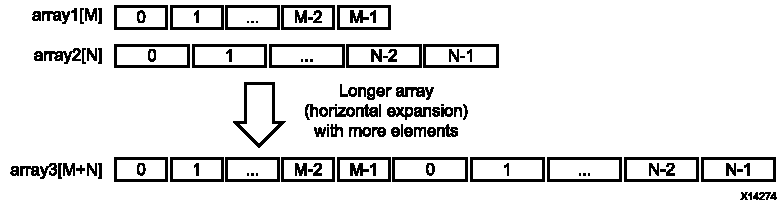
\includegraphics[scale=0.8]{./Figures/HLS7.pdf}
	\caption{Directiva ARRAY\_MAP en modo horizontal \citep{HLS2015}}
	\label{fig:HLS7}
\end{figure}

En la Figura \ref{fig:HLS10} se ve la aplicación en RAM de la directiva. Se puede notar que se toma una BRAM del tamaño de datos más ancho. Los bits sobrantes son descartados.

\begin{figure}[H]
	\centering
		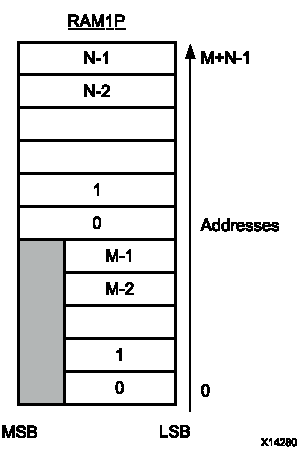
\includegraphics[scale=0.8]{./Figures/HLS10.pdf}
	\caption{Distribución en RAM del Mapeo Horizontal \citep{HLS2015}}
	\label{fig:HLS10}
\end{figure}

Implementaciones de este tipo traen complicaciones que pueden afectar de manera directa el rendimiento del circuito, pues dadas las grandes dimensiones y la limitada cantidad de puertos, se pueden presentar contenciones que darán lugar al efecto cuello de botella, donde la unidad de control deberá agendar los accesos a la RAM de tal forma que se extraigan los datos según la cantidad de peticiones.

\textbf{Mapeo Vertical:} Esta implementación consiste en la creación de un nuevo arreglo donde se concatenan los datos uno junto a otro; esto implica la creación de un arreglo de tamaño igual a la cantidad de datos individuales pero con un ancho de bits igual a la suma de los anchos de los arreglos a unir.

En la Figura \ref{fig:HLS8} se puede observar una representación del Mapeo Vertical; en este caso se han tomado dos arreglos de ancho e índices diferentes y se han concatenado elemento a elemento para formar un arreglo de mapeo vertical.

\begin{figure}[H]
	\centering
		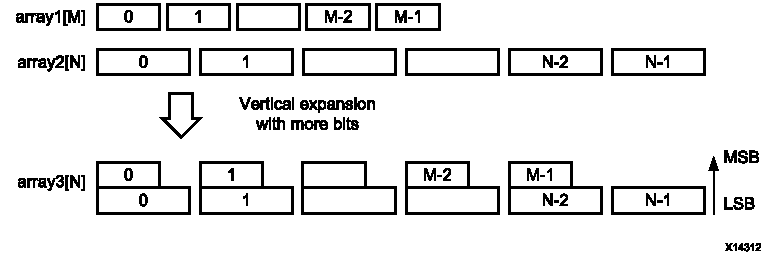
\includegraphics[scale=0.8]{./Figures/HLS8.pdf}
	\caption{Directiva ARRAY\_MAP en modo vertical \citep{HLS2015}}
	\label{fig:HLS8}
\end{figure}

El orden de concatenado se da a elección del diseñador, el cual le indica al sintetizador cuál subarreglo deberá ocupar la parte baja del elemento del arreglo y cuál la parte alta.

En la Figura \ref{fig:HLS11}, se aprecia cómo sería la distribución en la memoria RAM del mapeo vertical. En este caso, uno de los arreglos tiene mayor número de elementos que el otro y los bits restantes son puestos a tierra por el sintetizador.

\begin{figure}[H]
	\centering
		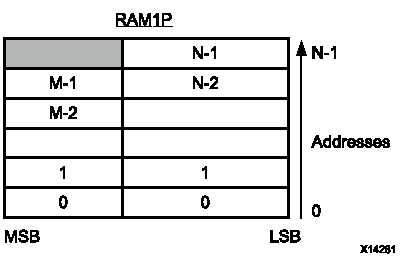
\includegraphics[scale=0.8]{./Figures/HLS11.pdf}
	\caption{Distribución en RAM del Mapeo Vertical  \citep{HLS2015}}
	\label{fig:HLS11}
\end{figure}

Otra de las directivas de Vivado HLS es la llamada ARRAY\_PARTITION. Esta directiva permite al programador incrementar el rendimiento del circuito cuando este se ve envuelto en un cuello de botella debido a las contenciones; esto se debe al número limitado de puertos con los que cuentan las memorias Block RAM de la FPGA y que el sistema intenta acceder simultáneamente a diferentes entradas que se encuentran en la misma memoria BRAM, como ocurre al aplicar la directiva PIPELINE.

\begin{figure}[H]
	\centering
		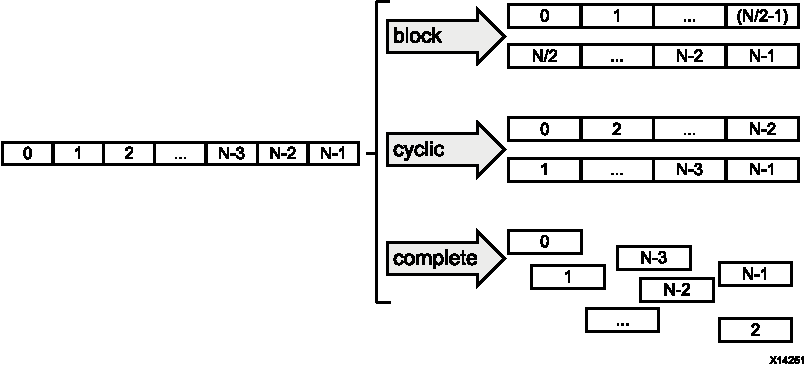
\includegraphics[scale=0.8]{./Figures/HLS5.pdf}
	\caption{Modos de operación de la directiva ARRAY\_PARTITION \citep{HLS2015}}
	\label{fig:HLS5}
\end{figure}

En la Figura \ref{fig:HLS5} se pueden observar los modos de operación de la directiva ARRAY\_PAR-\\TITION, los cuales se detallarán a continuación.

\begin{itemize}
\item \textbf{Bloque:} En este caso, el arreglo que se desea particionar será dividido en un número de acuerdo a un factor especificado por el diseñador y las necesidades del hardware.

\item \textbf{Cíclico:} Este modo permite particionar el arreglo de modo que se intercalen los índices del arreglo. En este modo también es posible adicionar un factor de partición.

\item \textbf{Completo:} En modo completo el sintetizador transformará el arreglo en registros individuales permitiendo acceder a cada elemento de forma individual; esto implica un aumento significativo de los recursos de hardware usados para cumplir el funcionamiento del circuito.
\end{itemize}

Continuando con el detalle de las directivas encontradas en Vivado HLS encontramos la directiva ARRAY\_RESHAPE, la cual es una combinación de  dos directivas anteriormente mencionadas: ARRAY\_MAP en modo vertical y ARRAY\_PARTITION. Esta directiva permite reducir el número de BRAM a usarse en la solución final y a su vez mantiene el beneficio de particionar los arreglos, cual es el acceso paralelo a los datos contenidos en la memoria.

La Figura \ref{fig:HLS12} nos muestra un ejemplo claro del funcionamiento de la directiva.

\begin{figure}[H]
	\centering
		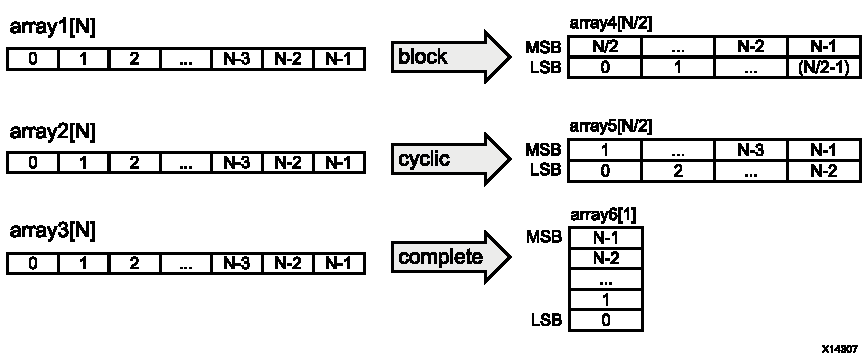
\includegraphics[scale=0.8]{./Figures/HLS12.pdf}
	\caption{Modos de operación de la Directiva ARRAY\_RESHAPE \citep{HLS2015}}
	\label{fig:HLS12}
\end{figure}

En este caso particular se han elegido tres arreglos diferentes de tamaño N; en ellos se ha elegido una partición en factor de dos para los modos BLOQUE y CICLICO. Como se mencionó anteriormente, cada uno de los elementos del índice se concatena usando el modo vertical del ARRAY\_MAP. En el caso del modo COMPLETO se concatena cada uno de los elementos para formar un solo elemento de ancho N, siendo el bit menos significativo el primer elemento del índice original y el bit más significativo el último bit del último elemento del índice original.

Dentro de las posibilidades de desarrollo usando síntesis de alto nivel con lenguajes como C/C++, surge la necesidad de adicionar el tipo de dato STRUCT o estructura; esto permite crear un tipo de dato el cual puede combinar diferentes tipos de datos en su interior. Estos datos no son más que referencias a posiciones de memoria, las cuales usan desplazamientos relativos (offsets) según el tipo de dato a acceder.

Sin embargo, a nivel de hardware, el acceso a los elementos individuales puede ser complejo dada la cantidad de elementos que la estructura puede contener. Por omisión, el sintetizador asume que cada arreglo dentro una estructura es una BRAM independiente, es por esto que se debe crear una lógica de control independiente para cada una de estas memorias.

En la Figura \ref{fig:HLS13} se observa el funcionamiento de la directiva DATA\_PACK, la cual permite optimizar el acceso a la estructura.

\begin{figure}[H]
	\centering
		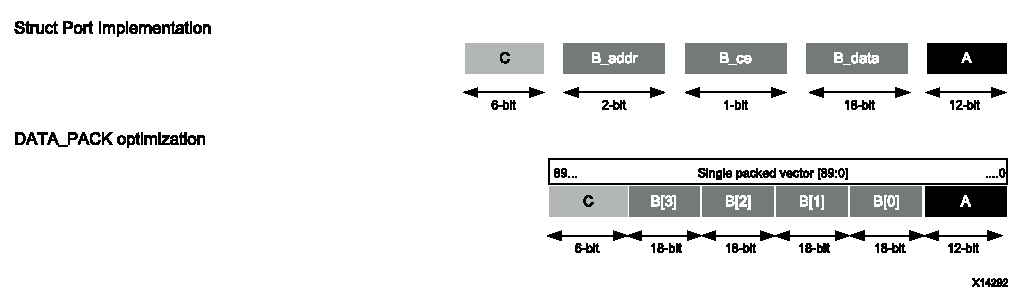
\includegraphics[scale=0.8]{./Figures/HLS13.pdf}
	\caption{Funcionamiento de la Directiva DATA PACK \citep{HLS2015}}
	\label{fig:HLS13}
\end{figure}

En este caso particular, el elemento A es un elemento individual de tipo int12, el elemento B es un arreglo de 4 elementos de tamaño int18 y finalmente el elemento C, es un elemento individual de tamaño int6. Como se infiere de la parte superior de la imagen, la implementación de la estructura implica que el sintetizador haga uso de dos LUT RAM para ocupar los elementos A y C y una BRAM para ocupar el elemento B con su respectiva lógica de control. Posterior a la optimización, es posible tener una sola BRAM conteniendo todos los elementos de la estructura; de esta forma, se puede reducir el hardware necesario para el funcionamiento del circuito reduciendo así la latencia del mismo.

Dentro de las posibilidades de realizar operaciones concurrentes con Vivado HLS podemos encontrar la directiva DATAFLOW. Esta directiva transforma el código de tal forma que es posible tener un paralelismo a nivel de tareas o procesos dentro del mismo algoritmo haciendo uso de pipeline.

En la Figura \ref{fig:HLS14} podemos apreciar el esquema de un circuito resuelto de manera secuencial usando funciones.

\begin{figure}[H]
  \centering
    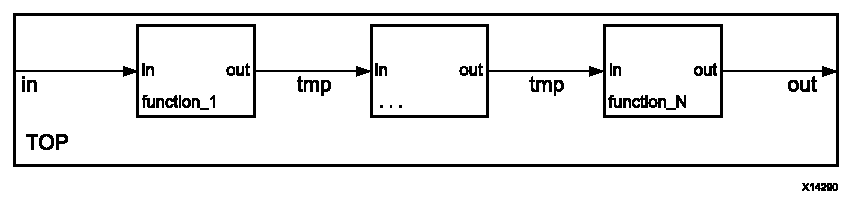
\includegraphics[scale=0.8]{./Figures/HLS14.pdf}
  \caption{Sistema secuencial  \citep{HLS2015}}
  \label{fig:HLS14}
\end{figure}

De esta forma es usual atacar la mayor cantidad de problemas si tienen una baja complejidad y cuentan con dependencias a nivel de datos como la variable \texttt{tmp} que se pasan las funciones en el módulo \texttt{TOP}.

Como se mencionó antes, la directiva DATAFLOW es capaz de transformar el código de tal forma que se crean canales de comunicación entre las diferentes funciones dividiendo las tareas entre procesos. Esto se puede observar en la Figura \ref{fig:HLS15}, donde la creación de los canales asegura que no se deba esperar a que termine la operación para continuar con las demás tareas.

\begin{figure}[H]
  \centering
    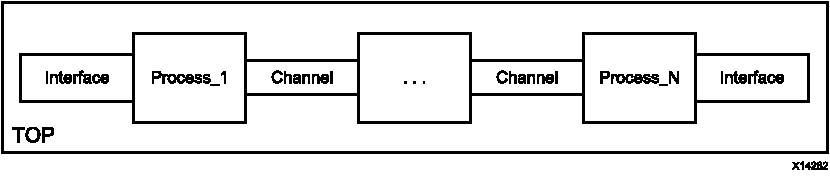
\includegraphics[scale=0.8]{./Figures/HLS15.pdf}
  \caption{Sistema concurrente a nivel de tareas \citep{HLS2015}}
  \label{fig:HLS15}
\end{figure}

En la Figura \ref{fig:HLS16} podemos ver un ejemplo claro del funcionamiento de la directiva DATAFLOW.

\begin{figure}[H]
  \centering
    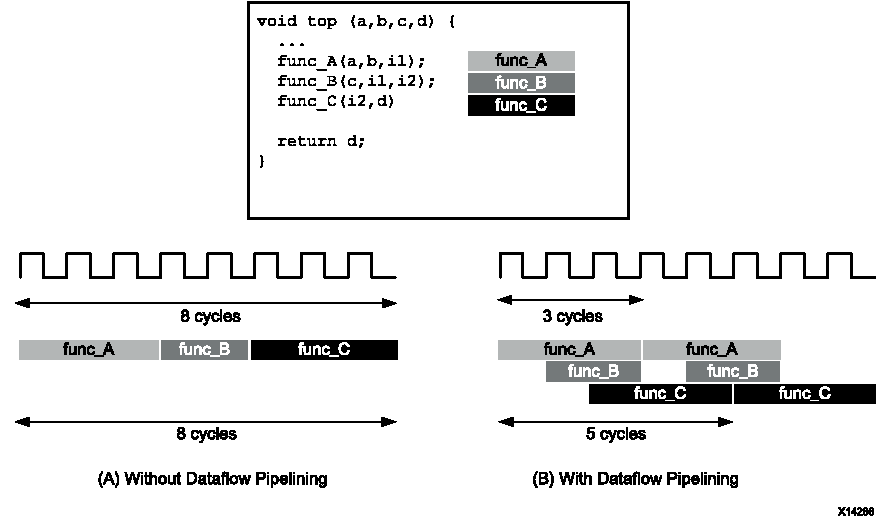
\includegraphics[scale=0.8]{./Figures/HLS16.pdf}
  \caption{Funcionamento de la directiva DATAFLOW \citep{HLS2015}}
  \label{fig:HLS16}
\end{figure}

En el lado (A) es posible ver cómo la operación tarda hasta 8 ciclos desde que se inicia la operación con \texttt{func\_A} y la salida del sistema \texttt{d} es escrita en memoria por \texttt{func\_C}. Usando la directiva DATAFLOW es posible aumentar la tasa a la que se obtienen resultados dada la operación en paralelo de las funciones usadas para calcular los resultados; en este caso, en el lado (B) vemos cómo el sistema es capaz de aceptar una nueva entrada al sistema cada 3 ciclos de reloj a diferencia de cada 8 ciclos sin la optimización y además, es posible obtener resultados cada 5 ciclos de reloj desde que ingresa un dato nuevo al circuito.

La directiva DATAFLOW requiere de condiciones específicas para garantizar la síntesis del circuito dentro de las cuales se deben cumplir los siguientes requerimientos:

\begin{itemize}
\item El sistema no debe tener ningún tipo de dependencia de datos.
\item Las funciones no deben tener retroalimentación.
\item Todas las funciones se deben ejecutar sin condiciones (\texttt{if}/\texttt{else}).
\item Los límites de los bucles deben ser fijos.
\item El sistema no puede tener paradas condicionales.
\end{itemize}

Vivado HLS es capaz de controlar la latencia de un bucle o una porción de código como tal; para esto es necesario usar la directiva LATENCY. Esta directiva restringe al sintetizador a alcanzar los valores de latencia indicados por el diseñador; en caso de no poder satisfacerlos, dadas las restricciones de hardware y propagación de los datos, el sintetizador tratará de alcanzar el nivel más bajo posible al indicado en el parámetro de la directiva.

Continuando con las mejoras en latencia de los circuitos usando Vivado HLS, podemos encontrar directivas como LOOP\_FLATTEN; esta directiva permite aplanar bucles anidados permitiendo reducir la latencia del bucle completo pues se elimina la lógica de control entre bucles.

La directiva LOOP\_FLATTEN requiere que el bucle a aplanar sea Perfecto o Semi-Perfecto; en el caso de ser un bucle imperfecto la directiva no será aplicada.

\begin{itemize}

\item \textbf{Bucle Anidado Perfecto:} Un bucle anidado perfecto es aquel en el cual no hay lógica entre bucles y únicamente el bucle más interior contiene lógica; además, los límites de los bucles son constantes.

\item \textbf{Bucle Anidado Semi-Perfecto:} Igual que el Bucle Anidado Perfecto, excepto porque los límites del bucle más externo pueden ser variables.

\end{itemize}

Además de la directiva de LOOP\_FLATTEN podemos encontrar la directiva LOOP \_MERGE. Esta directiva permite combinar bucles consecutivos no anidados e implica una mejora en la latencia general del sistema al reducir algunos ciclos de reloj entre la transición de bucles; este tiempo muerto se debe a que el circuito debe realizar una inicialización de variables, que por lo general no toma más de unos cuantos ciclos de reloj.

La Figura \ref{fig:HLS17} muestra un ejemplo de cómo una típica operación con dos bucles puede tener un impacto negativo en la ejecución del circuito.

\begin{figure}[H]
  \centering
    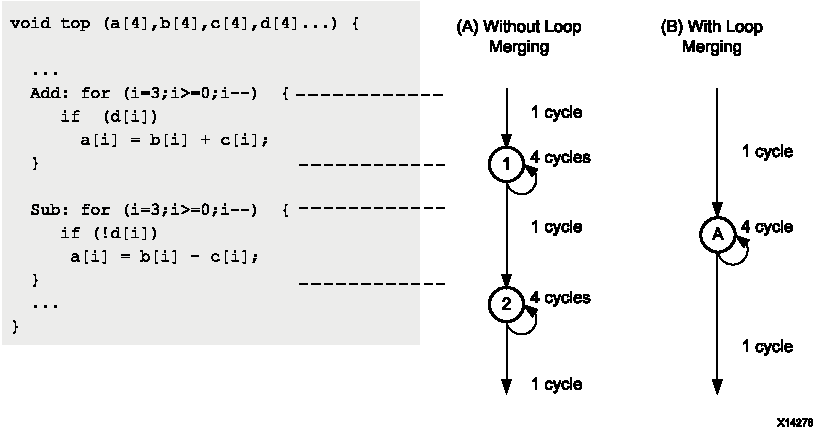
\includegraphics[scale=0.8]{./Figures/HLS17.pdf}
  \caption{Funcionamiento de la Directiva LOOP MERGE \citep{HLS2015}}
  \label{fig:HLS17}
\end{figure}

En este caso, sin la aplicación de la directiva, vemos que al sistema le toma 5 ciclos extra con respecto a aplicar la directiva al código fuente, pues se combinan ambos bucles en un solo estado de ejecución.

Es importante tener en cuenta que la directiva LOOP\_MERGE es únicamente aplicable si los bucles no cuentan con ningún tipo de dependencia entre sí.

La directiva PIPELINE provista por el software le da la posibilidad al diseñador de agregar etapas de pipeline a la ejecución de funciones y bucles dentro del código fuente del circuito a sintetizar; esta directiva se encarga de adicionar los estados de la unidad de control y el hardware necesario para el funcionamiento.

Como se describió anteriormente, la directiva PIPELINE puede ser aplicada tanto en funciones como en bucles. En la Figura \ref{fig:HLS18} se puede apreciar el comportamiento de la directiva aplicada a funciones en la parte izquierda y el comportamiento de la directiva aplicada a bucles en la parte derecha. En la parte inferior tenemos el comportamiento de las peticiones de lectura y escritura producido por ambas implementaciones. En el caso de aplicar la directiva a bucles, podemos notar que la unidad de control debe adicionar burbujas y liberar los registros cuando se requiere iniciar una nueva iteración del bucle. Esta, aunque es una operación necesaria, puede incrementar la latencia del circuito.

\begin{figure}[H]
  \centering
    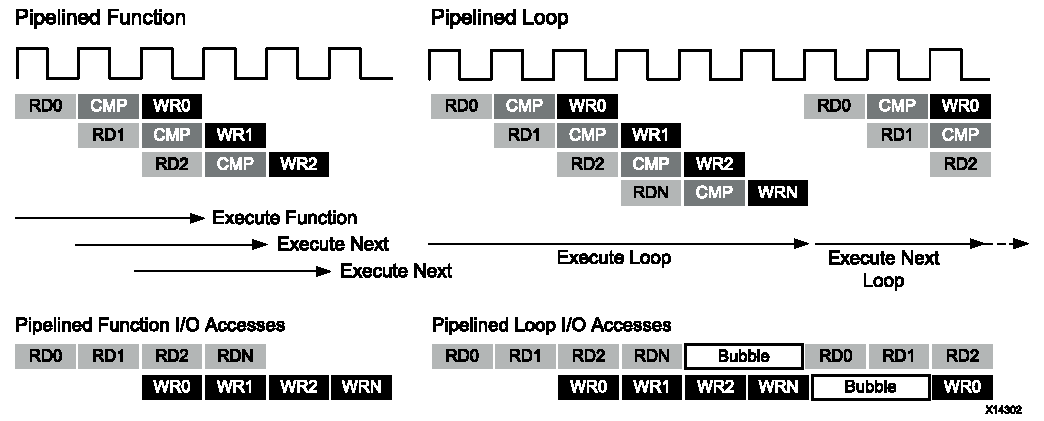
\includegraphics[scale=0.8]{./Figures/HLS18.pdf}
  \caption{Directiva PIPELINE aplicada a funciones y bucles \citep{HLS2015}}
  \label{fig:HLS18}
\end{figure}

La aplicación de la directiva PIPELINE provee al diseñador la capacidad de explotar en mayor medida el hardware que se está diseñando. Sin embargo, esta directiva trae consigo problemas como la adición de burbujas que claramente incrementan la latencia y el hecho de que el sistema deba desocupar el pipeline cuando los datos no estén disponibles para ser computados por el hardware; estos problemas pueden ser solucionados fácilmente con los modos PIPELINE\_REWIND y PIPELINE\_FLUSH respectivamente.

La Figura \ref{fig:HLS19} nos muestra el comportamiento de la directiva PIPELINE en su modo REWIND.

\begin{figure}[H]
  \centering
    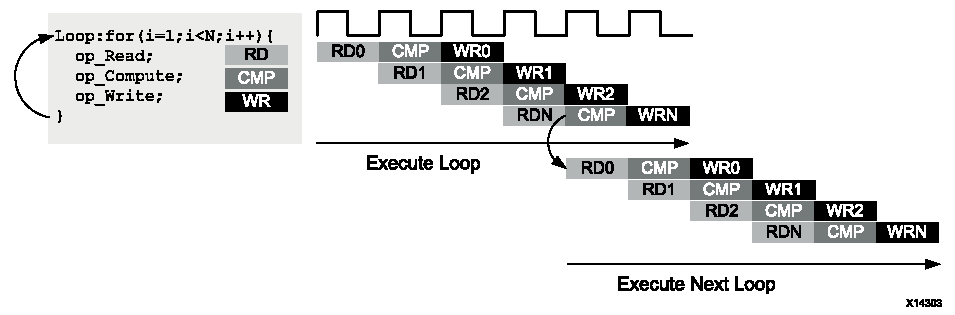
\includegraphics[scale=0.8]{./Figures/HLS19.pdf}
  \caption{Comportamiento del modo PIPELINE\_REWIND  \citep{HLS2015}}
  \label{fig:HLS19}
\end{figure}

Este modo permite reducir la latencia del circuito al ejecutar bucles, pues no requiere agregar burbujas ni evacuar las etapas del pipeline para continuar con la siguiente iteración. Este tipo de modos requiere una gran cantidad de hardware para su implementación y más aún cuando se realizan operaciones complicadas con bucles anidados. Es posible entonces que el sintetizador no pueda aplicar la directiva con este modo dada la complejidad y las dependencias de datos.

Otro de los problemas del pipeline es la dependencia de datos. La dependencia de datos cuando se corre un circuito con pipeline implica que este no puede continuar con las operaciones hasta que los datos se encuentren disponibles provocando que las etapas del pipe sean evacuadas. Esto trae consigo un incremento de la latencia, pues idealmente estas etapas deberían permanecer llenas. Con la aplicación del modo FLUSH de la directiva PIPELINE este tipo de eventos no provocará la evacuación de las etapas del pipeline, pues la unidad de control detecta el momento en que los recursos no se encuentran disponibles y congela la ejecución del hardware hasta que los datos se encuentran disponibles para ser computados nuevamente por el hardware; ver Figura \ref{fig:HLS3}.

\begin{figure}[H]
  \centering
    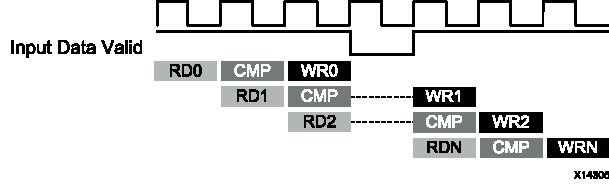
\includegraphics[scale=0.8]{./Figures/HLS3.pdf}
  \caption{Comportamiento del modo PIPELINE\_FLUSH \citep{HLS2015}}
  \label{fig:HLS3}
\end{figure}

Continuando con las directivas que favorecen la concurrencia encontramos la directiva UNROLL. Esta directiva permite dividir el hardware de un bucle especificando un factor de división. El factor de división de la directiva por omisión es un unroll de tamaño completo; ver Figura \ref{fig:HLS4}. Cada una de las divisiones que se realizan usando la directiva UNROLL crea instancias nuevas con los mismos recursos de hardware que el circuito original; la diferencia radica en la unidad de control y la forma en que se administra la ejecución del algoritmo usando las diferentes particiones; ver Figura \ref{fig:HLS4}.

\begin{figure}[H]
	\centering
		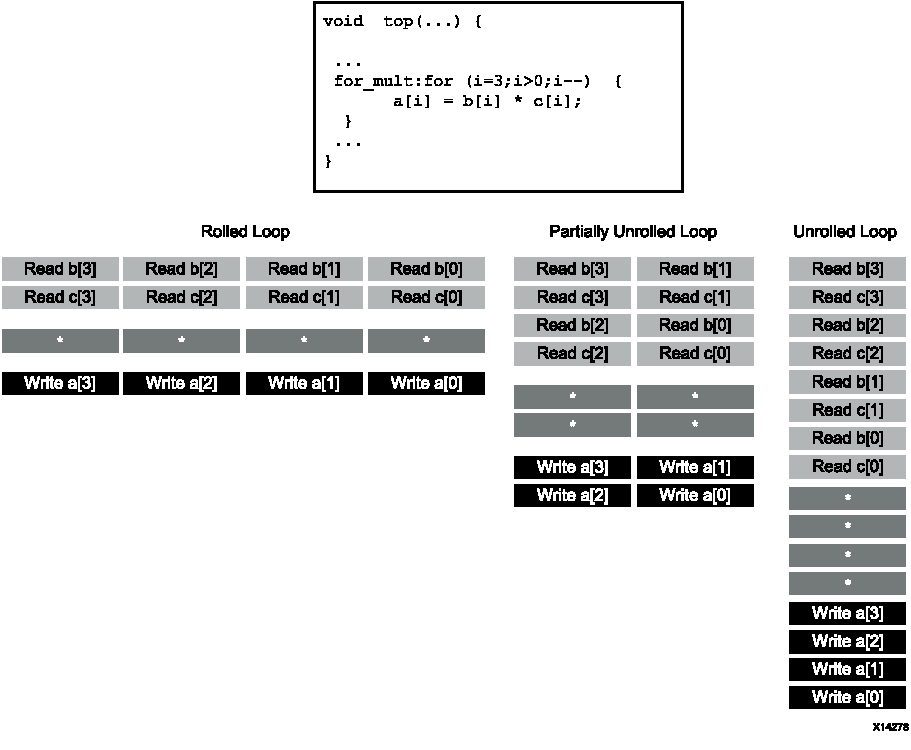
\includegraphics[scale=0.8]{./Figures/HLS4.pdf}
	\caption{Funcionamiento de la Directiva UNROLL \citep{HLS2015}}
	\label{fig:HLS4}
\end{figure}

Un bucle puede tener tres estados. El más común es el estado natural en el cual no se ha aplicado la directiva; este caso se conoce como un ROLLED LOOP. El segundo estado es aplicando la directiva con factor de dos o más; este estado se conoce como PARTIALLY UNROLLED LOOP. Finalmente el estado ideal, que implica consumir grandes cantidades de hardware es el FULLY UNROLLED LOOP; en este caso, cada una de las operaciones del circuito se realiza en un hardware dedicado.

La directiva UNROLL es capaz de reducir considerablemente la latencia del circuito tras su aplicación, pero su aplicación puede traer consecuencias como cuellos de botella si las memorias BRAM no han sido particionadas correctamente.

La directiva CLOCK es muy importante cuando se diseña usando HLS pues esta, permite al diseñador usar diferentes dominios de tiempo para cada uno de sus circuitos y funciones dentro del mismo módulo. Esto le da la libertad de validar el funcionamiento de su circuito con diferentes frecuencias de reloj, lo cual, si se aprovecha, puede incrementar el rendimiento general del circuito.

Finalmente, Vivado HLS cuenta con la directiva INLINE. Esta directiva le permite al programador expandir en línea funciones pequeñas dentro de aquellas que las llaman con mayor frecuencia, con lo cual, la aplicación de esta directiva elimina ciclos de establecimiento de señales entre funciones además de eliminar el hardware de control de las interfaces de las funciones.

La mayoría de herramientas de síntesis de alto nivel permite crear directivas múltiples por dominio, dando la posibilidad de aplicar una o más directivas a una porción de código específica. Por ejemplo, a un bucle podría aplicarse directivas de PIPELINE y UNROLL al mismo tiempo, lo cual incrementaría el performance de la aplicación. La única restricción de este tipo de modificaciones usando directivas son las dependencias de datos; este tipo de problemas podría evitar que la directiva sea aplicada correctamente por el sintetizador.

\section{Software de Síntesis de Hardware Vivado Design Suite}

Aplicaciones como Vivado HLS, además de la síntesis de alto nivel y simulación del hardware, no permiten una implementación final en la FPGA. Para este fin existen herramientas de síntesis de hardware como \href{http://www.xilinx.com/products/design-tools/vivado.html}{Vivado Design Suite} \citep{Vivad98}; este software transforma el código en VHDL arrojado por la síntesis de alto nivel en un bitstream, el cual contiene la configuración de la lógica de la FPGA. Vivado Design Suite es un software complejo que conoce la arquitectura de la FPGA y se encarga de los aspectos de la optimización final de tiempo, área y potencia de la implementación deseada.

En la Figura \ref{fig:HLS9} se puede ver un ejemplo claro de cómo el software interconecta los bloques IP Core. En hardware es común ver que un bloque IP tenga múltiples interfaces de entrada y salida. Por ejemplo, un módulo que desee interactuar con una memoria BRAM deberá contar con señales de control compatibles con dicha RAM; conectar individualmente estas señales implica tiempo y si se habla de interfaces más complejas como las interfaces AXI, que requieren de 45 señales en su formato FULL AXI4, la conexión requerirá aún más tiempo. Vivado Design Suite reconoce la interface de cada IP Core y las agrupa, permitiendo así realizar una sola conexión por interface.

\begin{figure}[H]
  \centering
    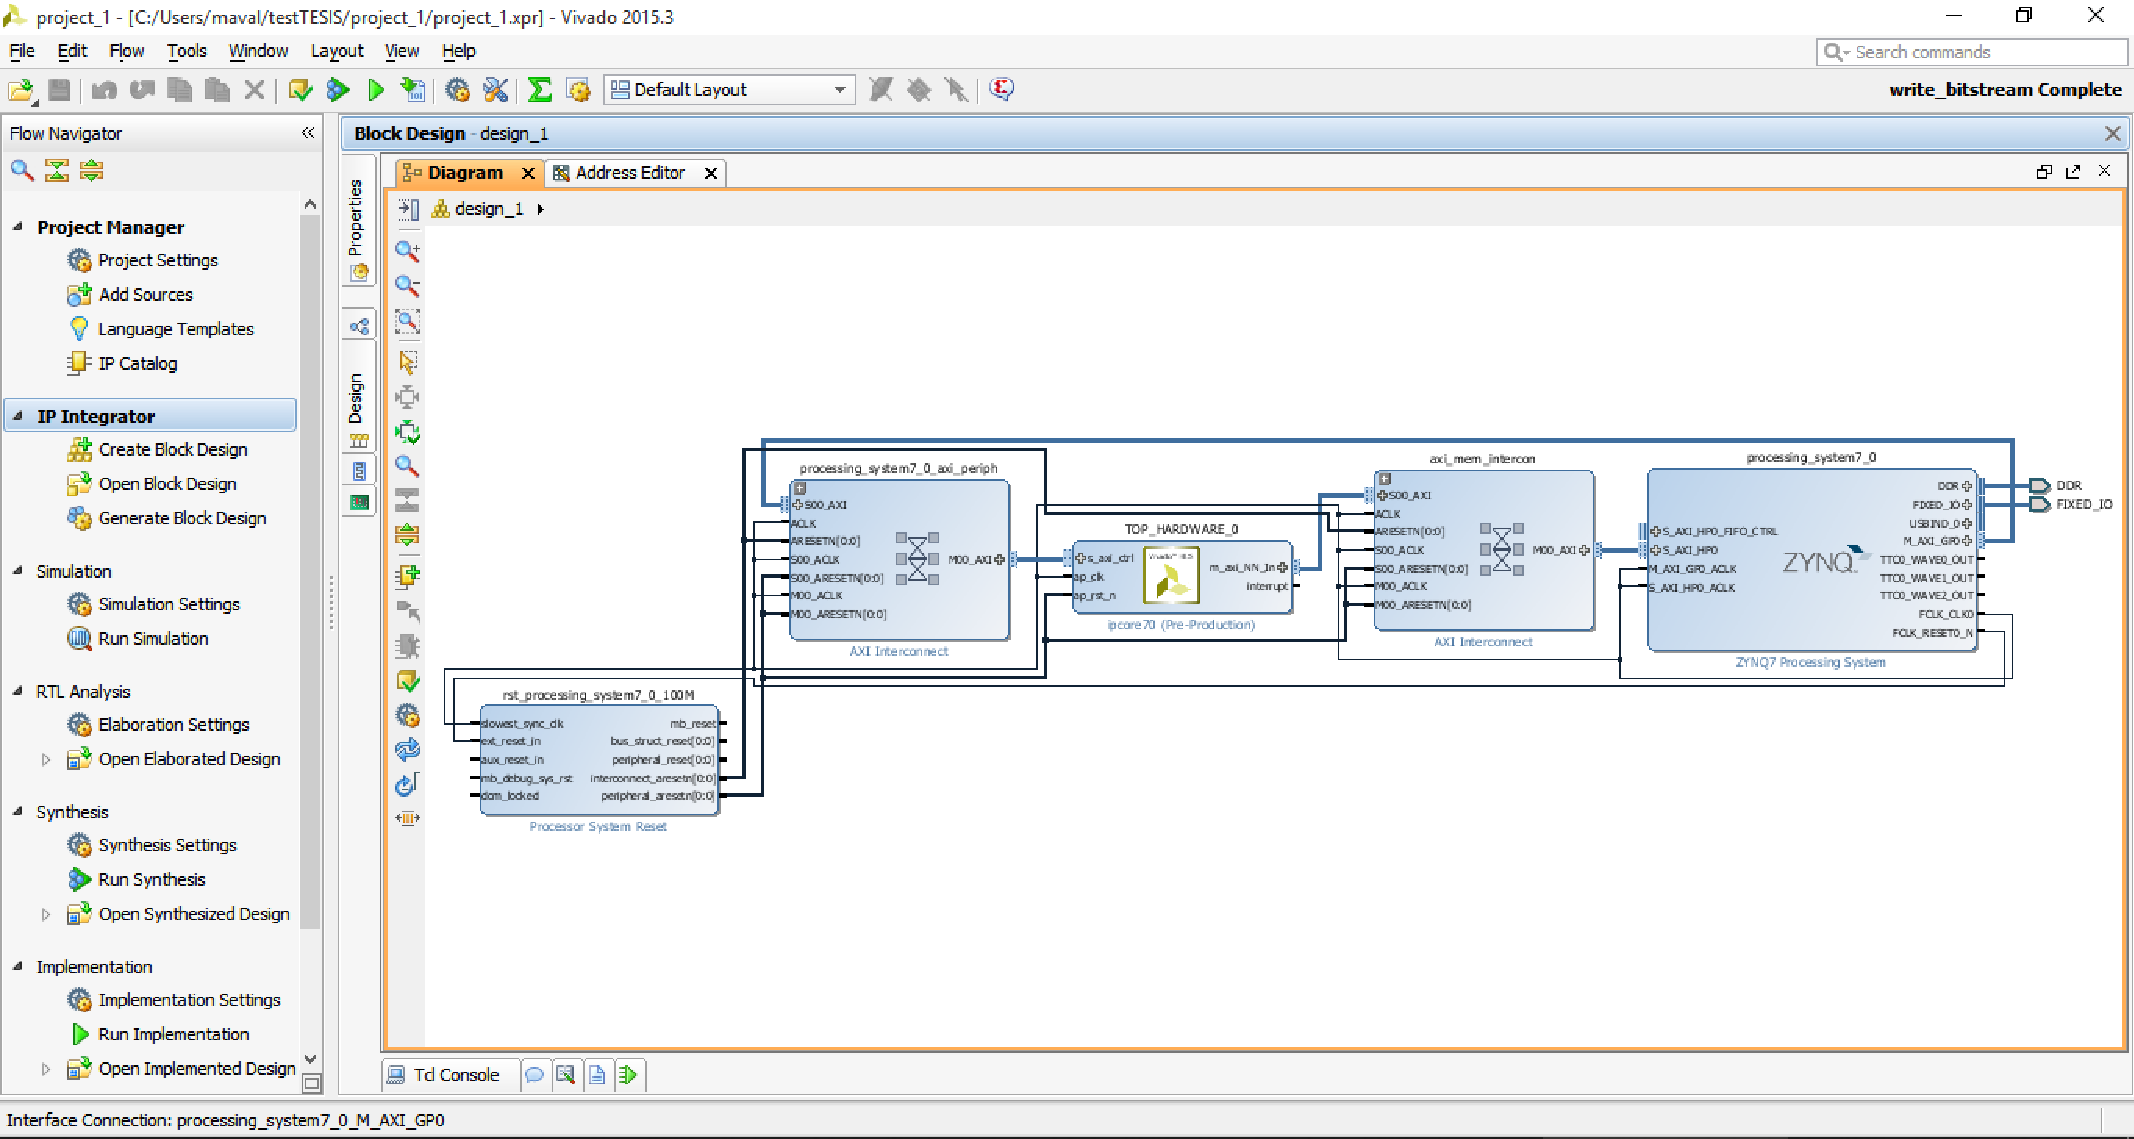
\includegraphics[scale=0.4]{./Figures/HLS9.pdf}
  \caption{Vivado Design Suite GUI}
  \label{fig:HLS9}
\end{figure}

En el caso de las interfaces mapeadas a memoria como las interfaces AXI, Vivado Design Suite se encarga de mostrarle al disenador el lugar de la memoria donde el sistema será mapeado; esto se hace según la Tabla \ref{tab:DIR}. Dependiendo del puerto al que se ha conectado el módulo al procesador ARM, quien es el que tiene el controlador de la memoria RAM DDR3, la herramienta entregará un rango de memoria disponible para el usuario.

% \begin{table}[H]
% \centering
% \begin{tabular}{|l|l|l|l|l|l|}
% \hline
% \textbf{Cell} & \textbf{Slave Interface} & \textbf{Base Name} & \textbf{Offset Address} & \textbf{Range} & \textbf{High Address} \\ \hline
% \multicolumn{6}{|l|}{processing\_system7\_0} \\ \hline
% \multicolumn{6}{|l|}{Data (32 address bits : 0x40000000 {[} 1G {]})} \\ \hline
% \multicolumn{6}{|l|}{M\_AXI\_GP0} \\ \hline
% TOPANN\_0 & s\_axi\_AXILiteS & Reg & 0x43C0\_0000 & 64K & 0x43C0\_FFFF \\ \hline
% \multicolumn{6}{|l|}{TOPANN\_0} \\ \hline
% \multicolumn{6}{|l|}{Data\_m\_axi\_INPUTS (32 address bits : 4G)} \\ \hline
% \multicolumn{6}{|l|}{m\_axi\_INPUTS} \\ \hline
% processing\_system7\_0 & S\_AXI\_HP0 & \begin{tabular}[c]{@{}l@{}}HP0\_DDR\_\\ LOWOCM\end{tabular} & 0x0000\_0000 & 512M & 0x1FFF\_FFFF \\ \hline
% \multicolumn{6}{|l|}{Data\_m\_axi\_OUTPUTS (32 address bits : 4G)} \\ \hline
% \multicolumn{6}{|l|}{m\_axi\_OUTPUTS} \\ \hline
% processing\_system7\_0 & S\_AXI\_HP0 & \begin{tabular}[c]{@{}l@{}}HP0\_DDR\_\\ LOWOCM\end{tabular} & 0x0000\_0000 & 512M & 0x1FFF\_FFFF \\ \hline
% \end{tabular}
% \caption{Mapeo de direcciones del Zynq 7000}
% \label{tab:DIR}
% \end{table}

\begin{table}[H]
\centering
\resizebox{\columnwidth}{!}{
\begin{tabular}{|l|c|c|c|l|}
\hline
\multicolumn{1}{|c|}{\textbf{Address Range}} & \textbf{CPUs y ACP} & \textbf{AXI\_HP} & \textbf{Others Bus Master} & \multicolumn{1}{c|}{\textbf{Notas}}                                                             \\ \hline
\multirow{4}{*}{0000\_0000 to 0003\_FFFF}   & OCM                 & OCM              & OCM                        & Address not filtered by SCU and OCM is mapped low                                               \\ \cline{2-5} 
                                            & DDR                 & OCM              & OCM                        & \begin{tabular}[c]{@{}l@{}}Address filtered by SCU and OCM is\\ mapped low\end{tabular}         \\ \cline{2-5} 
                                            & DDR                 &                  &                            & \begin{tabular}[c]{@{}l@{}}Address filtered by SCU and OCM is not\\ mapped low\end{tabular}     \\ \cline{2-5} 
                                            &                     &                  &                            & \begin{tabular}[c]{@{}l@{}}Address not filtered by SCU and OCM is\\ not mapped low\end{tabular} \\ \hline
\multirow{2}{*}{0004\_0000 to 0007\_FFFF}   & DDR                 &                  &                            & Address filtered by SCU                                                                         \\ \cline{2-5} 
                                            &                     &                  &                            & Address not filtered by SCU                                                                     \\ \hline
\multirow{2}{*}{0008\_0000 to 000F\_FFFF}   & DDR                 & DDR              & DDR                        & Address filtered by SCU                                                                         \\ \cline{2-5} 
                                            &                     & DDR              & DDR                        & Address not filtered by SCU                                                                     \\ \hline
0010\_0000 to 3FFF\_FFFF                    & DDR                 & DDR              & DDR                        & Accessible to all interconnect masters                                                          \\ \hline
4000\_0000 to 7FFF\_FFFF                    & PL                  &                  & PL                         & \begin{tabular}[c]{@{}l@{}}General Purpose Port \#0 to the PL,\\ M\_AXI\_GP0\end{tabular}       \\ \hline
8000\_0000 to BFFF\_FFFF                    & PL                  &                  & PL                         & \begin{tabular}[c]{@{}l@{}}General Purpose Port \#1 to the PL,\\ M\_AXI\_GP1\end{tabular}       \\ \hline
E000\_0000 to E02F\_FFFF                    & IOP                 &                  & IOP                        & I/O Peripheral registers                                                                        \\ \hline
E100\_0000 to E5FF\_FFFF                    & SMC                 &                  & SMC                        & SMC Memories                                                                                    \\ \hline
F800\_0000 to F800\_0BFF                    & SLCR                &                  & SLCR                       & SLCR registers                                                                                  \\ \hline
F800\_1000 to F880\_FFFF                    & PS                  &                  & PS                         & PS System registers                                                                             \\ \hline
F890\_0000 to F8F0\_2FFF                    & CPU                 &                  &                            & CPU Private registers                                                                           \\ \hline
FC00\_0000 to FDFF\_FFFF                    & Quad-SPI            &                  & Quad-SPI                   & Quad-SPI linear address for linear mode                                                         \\ \hline
\multirow{2}{*}{FFFC\_0000 to FFFF\_FFFF}   & OCM                 & OCM              & OCM                        & OCM is mapped high                                                                              \\ \cline{2-5} 
                                            &                     &                  &                            & OCM is not mapped high                                                                          \\ \hline
\end{tabular}
}
\caption{Mapa de Direcciones del Zynq 7000 Processing System \citep{TRM2017}}
\label{tab:DIR}
\end{table}

\section{Red Neuronal Artificial}

Las redes neuronales (\textit{ANN}, por las siglas en inglés de \textit{Artificial Neural Network}), han surgido como un mecanismo para solucionar problemas en diferentes ámbitos. Esto se debe a que estas tienen la capacidad de diagnosticar, detectar, predecir, monitorear, entre otras tareas \citep{amato2013artificial,singh2009artificial,sivapathasekaran2010artificial,kiani2010application}. La principal ventaja de estos sistemas es la facilidad que tienen para adaptarse a las necesidades de un problema. Solo se necesita un buen entrenamiento y una buena topología para que pueda cumplir con las exigencias del proyecto.

Para el desarrollo de ANN, existen dos técnicas muy conocidas, tanto para el entrenamiento como para la topología. La primera es \textit{BPA} \textit{(Back-Propagation Algorithm)}. Permite propagar el error de la salida por cada una de las capas de la red, de forma que el error de la salida se va reduciendo debido a la modificación de los pesos sinápticos. La segunda es \textit{MLP} \textit{(Multi-Layer Perceptron)}; esta es históricamente la más usada para el desarrollo de redes. Esto es debido a los buenos resultados que se han obtenido al implementarla \citep{wilamowski2009neural}.

\subsection{Neurona Básica}

Una neurona artificial o perceptrón es un modelo matemático basado en su contraparte biológica. Una neurona es una célula compuesta por una cantidad indefinida de conductos de entrada llamados dendritas y un conducto de salida llamado axón. Los conductos le permiten a la neurona comunicarse con otras neuronas, de forma que las señales de los sensores de entrada se van propagando a través de cada una. El perceptrón es la unidad de procesamiento básico de una ANN; está compuesto por cuatro partes esenciales: nodos de entrada, pesos sinápticos, función de propagación y función de salida, como se muestra en la Figura \ref{fig:neurona}.

\begin{figure}[H]
\centering
\begin{tikzpicture}[
cirt/.style={
  draw,
  circle,
  inner sep=2pt,
  font=\normalsize,
  join = by -latex
},
init/.style={
  draw,
  circle,
  inner sep=2pt,
  font=\Huge,
  join = by -latex
},
squa/.style={
  draw,
  inner sep=5pt,
  font=\Large,
  join = by -latex
}
]
\begin{scope}[start chain=1,node distance=13mm]
\node[on chain=1] at (0,1.5cm) 
  (x1) {$x_1$};
\node[on chain=1,cirt] 
  (w1) {$w_1$};
\end{scope}

\begin{scope}[start chain=2,node distance=13mm]
\node[on chain=2] at (0,0.5cm) 
  (x2) {$x_2$};
\node[on chain=2,cirt] 
  (w2) {$w_2$};
\end{scope}

\begin{scope}[start chain=3,node distance=13mm]
\node[on chain=3] at (0,-0.5cm) 
  (xp) {$\vdots$};
\node[on chain=3] 
  (wp) {$\vdots$};
\end{scope}

\begin{scope}[start chain=4,node distance=13mm]
\node[on chain=4] at (0,-1.5cm) 
  (xn) {$x_n$};
\node[on chain=4,cirt,label=below:{\parbox{2cm}{\centering Pesos \\ sinápticos}}] 
  (wn) {$w_n$};
\end{scope}

\begin{scope}[start chain=5,node distance=13mm]
\node[on chain=5,init] at (4cm,0) (sigma) 
  {$\displaystyle\Sigma$};
\node[on chain=5,squa,label=above:{\parbox{2cm}{\centering Función de \\ activación}}](f){$\varphi(u)$};
\node[on chain=5,label=above:Salida,join=by -latex] (y)
  {$y$};
\end{scope}

\node[label=above:\parbox{2cm}{\centering Bias}] at (sigma|-w1) (b) {$\theta$};

\draw[-latex] (w1) -- (sigma);
\draw[-latex] (w2) -- (sigma);
\draw[-latex] (wn) -- (sigma);
\draw[-latex] (b) -- (sigma);
\draw[-latex] (sigma) to [edge node={node [sloped,above] {$u$}}] (f);
\draw[decorate,decoration={brace,mirror,amplitude=10pt}] (x1.north west) -- node[left=10pt] {Entradas} (xn.south west);
\end{tikzpicture}
\caption{Neurona básica}
\label{fig:neurona}
\end{figure}

\subsubsection{Función de Propagación}

Para el modelo matemático, las señales de entrada son expresadas por el conjunto $X=(x_1, x_2, x_3, \ldots, x_n)^T$. Para simular el proceso de reorganización de las conexiones sinápticas de las neuronas biológicas, se asocia a cada elemento del conjunto de entrada un peso sináptico que le permite darle a la conexión un valor de excitación o de inhibición dependiendo del signo. Los pesos sinápticos se expresan por el conjunto $W=(w_1, w_2, w_3, \ldots, w_n)^T$.

La función de propagación se encarga de multiplicar el conjunto de entrada y el conjunto de pesos sinápticos, término a término, para luego hacer la sumatoria de los elementos del vector resultante y así generar un valor de salida, $u$. La expresión completa para la función de propagación está dada por la Ecuación \ref{eq:funpro}

\begin{equation}\label{eq:funpro}
  u=\sum_{i=1}^{n} w_ix_i + \theta
\end{equation}

donde $x_i \in X$, $w_i \in W$ y $\theta$ es el umbral de inhibición o excitación de la neurona.

\subsubsection{Función de  Activación}

La función de activación surge como una necesidad de tener una salida de la neurona acotada a un rango determinado; esto se debe a que la salida en la neurona biológica se encuentra acotada en amplitud. En la Ecuación \ref{eq:func} se muestra la expresión matemática respecto a $u$.

\begin{equation}\label{eq:func}
  y=\varphi(u)
\end{equation}

Existen diferentes tipos de funciones de activación. La elección de estas depende del objetivo del diseño:

\begin{table}[H]
\centering 
\renewcommand{\arraystretch}{1.8}
\begin{tabular}{| >{\centering\arraybackslash}m{2.4cm} | >{\arraybackslash}m{6cm}|}
\hline %inserts horizontal line
\textbf{Función de Activación} & \textbf{Expresión Matemática}\\ 
\hline 
Paso Unitario & $\varphi(u) = \begin{cases} 1.0 &\mbox{si } u > 0 \\ 
0.0 & \mbox{en otros casos}. \end{cases}$\\  \hline 
Rampa & $\varphi(u) = max \lbrace 0.0, min \lbrace 1.0, u+0.5 \rbrace \rbrace$\\ \hline 
Sigmoidal & $\varphi(u) = \dfrac{1}{1+e^{-u}}$\\ \hline 
Bipolar Sigmoid & $\varphi(u) = \dfrac{1-e^{-u}}{1+e^{-u}}$\\ \hline 
Tangente Sigmoidal & $\varphi(u) = \dfrac{2}{1+e^{-2u}}-1$\\ \hline 
\end{tabular}
\caption{Funciones de Activación}
\label{tab:funactivacion}
\end{table}

\subsection{Perceptrón Multi-Capa}

Un MLP \textit{Multilayer Perceptron} es una red de neuronas que está compuesta por una capa de nodos de entrada, una o dos capas ocultas y una capa de salida. Todas las capas están compuestas por neuronas artificiales a excepción de la capa de entrada donde los nodos son las señales de ingreso a la red. Las conexiones entre capas dependen de la configuración de la red; puede ser completamente conectada si cada uno de los nodos de una capa se conecta con todos los nodos de la siguiente, véase Figura \ref{fig:MLP}. Por otro lado, puede tener una conexión personalizada y no estar completamente conectada.

\begin{figure}[H]
\centering
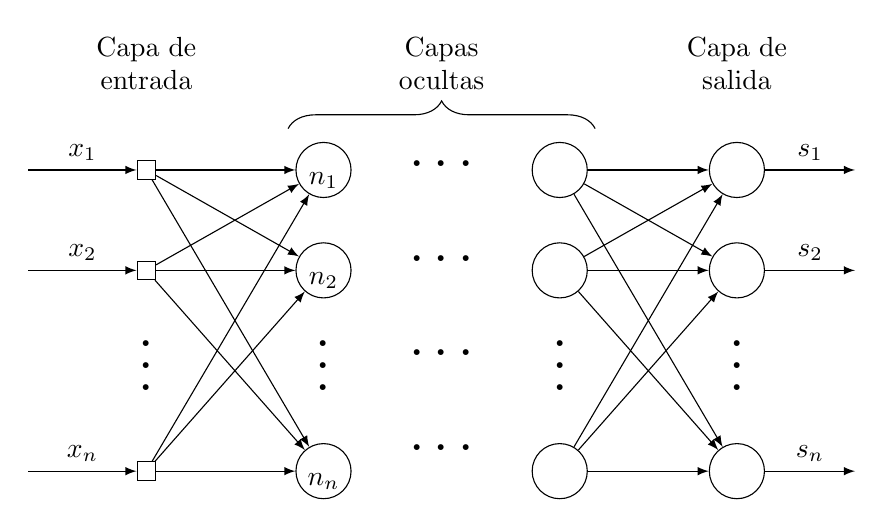
\begin{tikzpicture}[x=1.5cm, y=1.5cm,
every neuron/.style={
    circle,
    draw,
    minimum size=0.7cm
  },
every input/.style={
    draw,
  },
every layer/.style={
    draw=none, 
    scale=2,
    execute at begin node=\color{black}$\ldots$
  },
neuron missing/.style={
    draw=none, 
    scale=2,
    text height=0.25cm,
    execute at begin node=\color{black}$\vdots$
  }
]
\foreach \m/\l [count=\y] in {1,2,missing,3}
  \node [every input/.try, neuron \m/.try] (input-\m) at (0,2.5-\y*0.85) {};

\foreach \m [count=\y] in {1,2,missing,3}
  \node [every neuron/.try, neuron \m/.try ] (hidden1-\m) at (1.5,2.5-\y*0.85) {};

\foreach \m [count=\y] in {1,2,3,4}
  \node [every layer/.try] (empty-\m) at (2.5,2.5-\y*0.8) {};
  
  \foreach \m [count=\y] in {1,2,missing,3}
  \node [every neuron/.try, neuron \m/.try ] (hidden2-\m) at (3.5,2.5-\y*0.85) {};

\foreach \m [count=\y] in {1,2,missing,3}
  \node [every neuron/.try, neuron \m/.try ] (output-\m) at (5,2.5-\y*0.85) {};

\foreach \l [count=\i] in {1,2,n}
  \draw [latex-] (input-\i) -- ++(-1,0)
    node [above, midway] {$x_\l$};

\foreach \l [count=\i] in {1,2,n}
  \node [above] at (hidden1-\i.south) {$n_\l$};

\foreach \l [count=\i] in {1,2,n}
  \draw [-latex] (output-\i) -- ++(1,0)
    node [above, midway] {$s_\l$};

\foreach \i in {1,...,3}
  \foreach \j in {1,...,3}
    \draw [-latex] (input-\i) -- (hidden1-\j);

\foreach \i in {1,...,3}
  \foreach \j in {1,...,3}
    \draw [-latex] (hidden2-\i) -- (output-\j);

\node [align=center, above] at (0,2.25) {Capa de \\ entrada};
\node [align=center, above] at (2.5,2.25) {Capas \\ ocultas};
\node [align=center, above] at (5,2.25) {Capa de \\ salida};
\draw [decorate,decoration={brace,amplitude=10pt}] (1.2,2) -- (3.8,2);
\end{tikzpicture}
\caption{MLP completamente conectada}
\label{fig:MLP}
\end{figure}